\section{Unsupervised consensus maximization}

Consensus maximization in a set of features related by a geometric constraint that also contains outliers is an important aspect of an SFM system. The problem consists of finding the largest set of inlier features that is consistent with a geometric constraint. In a 3D vision setting the geometric constraint could be for example a rigid transformation $[\textbf{R}\ \textbf{t}]$, a fundamental matrix $\textbf{F}$ or a homography $\textbf{H}$ that relates pairs of corresponding 3D or 2D points.

A popular algorithm to solve this problem is RANSAC\cite{ransac}, which is a classical iterative method. On the other hand, an unsupervised machine learning method for consensus maximization is presented in another paper\cite{consensus}. The explanation of the method in the original paper uses very strict group theory. This section of the thesis will instead try to explain the method with emphasis on ease of understanding and not be as strict on the theory. The focus will be on explaining the method used to extract the parameters of the constraint, as it is not explained by the original paper in detail and took a lot of figuring out on my part, especially how to extract the parameters of the homography.

Consider one of the simplest geometric constraints on a set of corresponding 2D points in subsequent frames of the KITTI dataset, the fundamental matrix $\textbf{F}$. Given 8 or more points, the fundamental matrix can be calculated using the 8-point algorithm\cite{8-point}. Considering a point $\textbf{u}$ in frame 1, and point $\textbf{v}$ in frame 2 the relationship between them can be expressed in the following way.

 \begin{equation}
 \textbf{u}^T \textbf{F} \textbf{v} = 0
 \end{equation}
 
 To be more explicit the relation can be expressed as follows.
 
\begin{equation}
\begin{pmatrix}
u_\mathrm{x} & u_\mathrm{y} & 1 \\
\end{pmatrix}
\begin{pmatrix}
f_{11} & f_{12} & f_{13} \\
f_{21} & f_{22} & f_{23} \\
f_{31} & f_{32} & f_{33} \\
\end{pmatrix}
\begin{pmatrix}
v_\mathrm{x} \\
v_\mathrm{y} \\
1 \\
\end{pmatrix}
= 0
\end{equation}

Multiplication of the two rightmost matrices gives:

\begin{equation}
\begin{pmatrix}
u_\mathrm{x} & u_\mathrm{y} & 1 \\
\end{pmatrix}
\begin{pmatrix}
f_{11} v_\mathrm{x} + f_{12} v_\mathrm{y} + f_{13} \\
f_{21} v_\mathrm{x} + f_{22} v_\mathrm{y} + f_{23} \\
f_{31} v_\mathrm{x} + f_{32} v_\mathrm{y} + f_{33} \\
\end{pmatrix}
= 0
\end{equation}

Multiplication of the remaining two matrices and grouping $\textbf{u}$ and $\textbf{v}$ in parentheses for readability gives the following linear equation.

\begin{equation}
f_{11} (u_\mathrm{x} v_\mathrm{x}) + f_{12} (u_\mathrm{x} v_\mathrm{y}) + f_{13} (u_\mathrm{x}) +
f_{21} (u_\mathrm{y} v_x) + f_{22} (u_\mathrm{y} v_\mathrm{y}) + f_{23} (u_\mathrm{y}) +
f_{31} (v_\mathrm{x}) + f_{32} (v_\mathrm{y}) + f_{33} (1)
= 0
\end{equation}

Now consider a set of $m$ corresponding points that are related by the same fundamental matrix $\textbf{F}$. Place the 9 monomials in the parentheses for all $m$ points in a matrix $\textbf{M} \in \mathbb{R}^{mx9} $, we call this a monomial matrix. A monomial is an expression in algebra that contains only one term.

\begin{equation}
\mathbf{M}=
\begin{pmatrix}
u_{\mathrm{x},1} v_{\mathrm{x},1} & u_{\mathrm{x},1} v_{\mathrm{y},1} & u_{\mathrm{x},1} & u_{\mathrm{y},1} v_{\mathrm{x},1} & u_{\mathrm{y},1} v_{\mathrm{y},1} & u_{\mathrm{y},1} & v_{\mathrm{x},1} & v_{\mathrm{y},1} & 1 \\
 & & & \vdots & & & & & \\
u_{\mathrm{x},m} v_{\mathrm{x},m} & u_{\mathrm{x},m} v_{\mathrm{y},m} & u_{\mathrm{x},m} & u_{\mathrm{y},m} v_{\mathrm{x},m} & u_{\mathrm{y},m} v_{y,m} & u_{\mathrm{y},m} & v_{\mathrm{x},m} & v_{\mathrm{y},m} & 1 \\
\end{pmatrix}
\end{equation}

The constraint is satisfied by all $m$ points if

\begin{equation}
\textbf{M}
\begin{pmatrix}
f_{11} \\
f_{12} \\
f_{13} \\
f_{21} \\
f_{22} \\
f_{23} \\
f_{31} \\
f_{32} \\
f_{33} \\
\end{pmatrix}
=
\begin{pmatrix}
0 \\
\vdots \\
0 \\
\end{pmatrix}
^{mx1}
\end{equation}

Now the solution $\textbf{f}$ should look very familiar. The column vector $\textbf{f}$ is in fact the very definition of a nullspace of $\mathbf{M}$. This is the key insight in this method of unsupervised consensus maximization. Finding the nullspace of $\mathbf{M}$ is done by performing a singular value decomposition, which is a differentiable operation.

\begin{equation}
\mathbf{U}\mathbf{\Sigma}\mathbf{V}^T=\mathbf{M}
\end{equation}

The nullspace will be the last column vector of $\mathbf{V} \in \mathbb{R}^{9x9}$ and the last singular value $\sigma_9$ in the diagonal of $\mathbf{\Sigma}$ will be zero. This is correct only if the set of corresponding points contains only inliers. If the set contains outliers that can not be related by the geometric constraint then the last singular value $\sigma_9$ will be greater than zero. If the inliers and outliers were known they could be represented by a vector $\textbf{w} \in [0,1]^m$ where $ 1 $ means inlier and $ 0 $ means outlier. Now $\mathbf{M}$ can be weighted by $\textbf{w}$ which would cancel all rows in $\mathbf{M}$ which come from an outlier pair of points.

\[
\diag(\textbf{w}) \mathbf{M} \textbf{f} = \textbf{0}
\] 

The problem of finding the largest set of inliers has now been transformed into finding the weights $\textbf{w}$ such that the last singular value $\sigma_9$ of $\diag(\textbf{w})\mathbf{M}$ is near zero, and the sum of the weights should also be large to have as many inliers as possible.

To learn the weight $w_i \in \textbf{w}$ for each pair of points, the PointNet\cite{pointnet} architecture was used. The pair of points are concatenated into rows of a $\mathbf{X}\in \mathbb{R}^{m\times n} $ matrix. For 2D points $n = 2+2=4$ and for 3D points $n=3+3=6$. The input $\mathbf{X}$ is fed trough the PointNet segmentation network with a single output class, signifying if the point pair is an inlier or not. The key innovation of the PointNet architecture is that it can directly consume point cloud data, as opposed to first transforming the input to a 3D voxel grid or an image. The network is also invariant to the ordering of the points in the input list. Figure \ref{fig:consensus} illustrates the process of feeding the input through PointNet to get the weights, and then applying the weights to the monomial matrix of which we want to minimize the last singular value.

\begin{figure}[H]
	\centering
	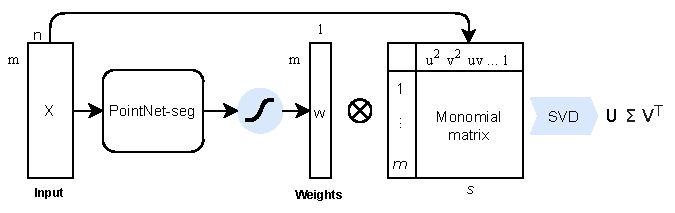
\includegraphics[width=1.0\textwidth]{consensus}
	\caption{The input point positions $\mathbf{X}\in \mathbb{R}^{m\times n}$ are fed trough the PointNet segmentation network, and are also used to construct the monomial matrix $\mathbf{M}$. The rows of $\mathbf{M}$ are weighted using the weights $\mathbf{w}$. The network learns to predict inliers by minimizing the last singular values in $\mathbf{\Sigma}$ in the loss function.}
	\label{fig:consensus}
\end{figure}

Because the fundamental matrix is a constraint expressed by one linear equation a basis of only one  nullspace vector is needed from the singular value decomposition to construct it. But the method can also be used to learn constraints such as a homography or rigid 3D transformation that are constrained by 3 linear equations and therefore require a basis of 3 nullspace vectors. In that case the last 3 singular values from the SVD should be minimized in the loss function.

In the following sections the method used to extract the homography from the basis vectors will be explained. Two points that are related by a homography is expressed as follows. The monomials are grouped by parentheses.

\begin{equation}
\mathbf{u} \times \mathbf{H}\mathbf{v}=0 \rightarrow
\label{eqn:H-cross}
\end{equation}
\begin{equation}
[\mathbf{u}]_{\times} \mathbf{H}\mathbf{v}=0 \rightarrow
\end{equation}
\begin{equation}
\begin{pmatrix}
0 & -1 & u_\mathrm{y} \\
1 & 0 & -u_\mathrm{x} \\
-u_\mathrm{y} & u_\mathrm{x} & 0 \\
\end{pmatrix}
\begin{pmatrix}
h_{11} & h_{12} & h_{13} \\
h_{21} & h_{22} & h_{23} \\
h_{31} & h_{32} & h_{33} \\
\end{pmatrix}
\begin{pmatrix}
v_\mathrm{x} \\
v_\mathrm{y} \\
1 \\
\end{pmatrix}
=
\begin{pmatrix}
0 \\
0 \\
0 \\
\end{pmatrix}
\rightarrow
\end{equation}
\begin{equation}
-h_{21} (v_\mathrm{x}) \ \ \ \ - h_{22} (v_\mathrm{y}) \ \ \ \ - h_{23} (1) \ \ \ + h_{31} (v_\mathrm{x} u_\mathrm{y}) + h_{32} (v_\mathrm{y} u_\mathrm{y}) + h_{33} (u_\mathrm{y}) = 0 \\
\label{eqn:H-1}
\end{equation}
\begin{equation}
\ \ h_{11} (v_\mathrm{x}) \ \ \ \ \ + h_{12} (v_\mathrm{y}) \ \ \ \ + h_{13} (1) \ \ \ -h_{31} (v_\mathrm{x} u_\mathrm{x}) -h_{32} (v_\mathrm{y} u_\mathrm{x}) - h_{33} (u_\mathrm{x}) = 0 \\
\label{eqn:H-2}
\end{equation}
\begin{equation}
-h_{11} (v_\mathrm{x} u_\mathrm{y}) -h_{12} (v_\mathrm{y} u_\mathrm{y}) -h_{13} (u_\mathrm{y}) + h_{21} (v_\mathrm{x} u_\mathrm{x}) + h_{22} (v_\mathrm{y} u_\mathrm{x}) + h_{23} (u_\mathrm{x}) = 0 \\
\label{eqn:H-3}
\end{equation}

Note that the above derivation (\ref{eqn:H-cross}-\ref{eqn:H-3}) is identical to the DLT algorithm\cite{Hartley2004}. The monomials in the parentheses are the same as for the fundamental constraint, which means that the same monomial matrix $\textbf{M}$ can be used. But because a homography is constrained by $r=3$ linear equations, the last three singular values of the SVD should be minimized during training. Extract three basis vectors from the nullspace which will be the three rightmost columns of $\textbf{V}$ in the SVD of $\diag(\textbf{w})\textbf{M}$.

\begin{equation}
\mathbf{B} = 
\begin{pmatrix}
\textbf{v}_7 & \textbf{v}_8 & \textbf{v}_9
\end{pmatrix}
\in \mathbb{R}^{9x3}
\end{equation}

When calculating the fundamental matrix, the nullspace of the monomial matrix had a direct one to one mapping with the parameters needed to construct $\textbf{F}$. This is no longer the case when we want to use the nullspace basis $\textbf{B}$ to construct the homography matrix $\textbf{H}$. This is because the 3 linear equations of $H$ are tangled. Notice that $h_{21}$, $h_{22}$ and $h_{23}$ appear both in equation \ref{eqn:H-1} and \ref{eqn:H-3}. Also $h_{31}$, $h_{32}$ and $h_{33}$ appear both in equation \ref{eqn:H-1} and \ref{eqn:H-3}. Also $h_{11}$, $h_{12}$ and $h_{13}$ appear both in equation \ref{eqn:H-2} and \ref{eqn:H-3}. In order to extract the elements of $\textbf{H}$ from the nullspace basis vectors in $\textbf{B}$ we need to perform a change of basis.
Notice that equation \ref{eqn:H-1} does not contain $u_\mathrm{x}$ and equation \ref{eqn:H-2} does not contain $u_\mathrm{y}$. We can exploit this fact to perform a change of basis on $\textbf{B} \in \mathbb{R}^{9x3}$ to get $\textbf{B}' \in \mathbb{R}^{9x2}$ that should have the structure seen in Table \ref{table:H}.

\begin{table}[H]
\centering
\begin{tabular}{ c c c }
	Monomial & Structure of $\textbf{B}'$ & Corresponding element in $\textbf{H}$ \\
	$u_\mathrm{x} v_\mathrm{x}$ & \multirow{9}{*}{
$\begin{pmatrix}
	0 & . \\
	0 & . \\
	0 & . \\
	. & 0 \\
	. & 0 \\
	. & 0 \\
	. & . \\
	. & . \\
	. & . \\
\end{pmatrix}$
} & \multirow{9}{*}{
$\begin{pmatrix}
 & h_{31} \\
 & h_{32} \\
 & h_{33} \\
h_{31} &   \\
h_{32} &   \\
h_{33} &   \\
h_{21} & h_{11} \\
h_{22} & h_{12} \\
h_{23} & h_{13} \\
\end{pmatrix}$
} \\
	$u_\mathrm{x} v_\mathrm{y}$ & \\
	$u_\mathrm{x} \ \ \ \ $ & \\    
	\hline
	$u_\mathrm{y} v_\mathrm{x}$ & \\
	$u_\mathrm{y} v_\mathrm{y}$ & \\
	$u_\mathrm{y} \ \ \ \ $ & \\    
	\hline
	$\ \ \ \ v_\mathrm{x}$ & \\
	$\ \ \ \ v_\mathrm{y}$ & \\
	$\ \ \ \ 1$ & \\
\end{tabular}
\caption{The basis monomials, the structure of $\textbf{B}'$ in the new basis and its corresponding elements in $\textbf{H}$.}
\label{table:H}
\end{table}

To perform the change of basis to get the structure of $\textbf{B}'$ we use the nullspace $\textbf{n}_1 \in \mathbb{R}^{3\times 1}$ of rows 1, 2 and 3 from $\textbf{B}$, and the nullspace $\textbf{n}_2 \in \mathbb{R}^{3x1}$ of row 4, 5, 6 from $\textbf{B}$.

\begin{equation}
\textbf{A}_1 = 
\begin{pmatrix}
b_{11} & b_{12} & b_{13} \\
b_{21} & b_{22} & b_{23} \\
b_{31} & b_{32} & b_{33} \\
\end{pmatrix},
\textbf{A}_2 = 
\begin{pmatrix}
b_{41} & b_{42} & b_{43} \\
b_{51} & b_{52} & b_{53} \\
b_{61} & b_{62} & b_{63} \\
\end{pmatrix}
\end{equation}
\begin{equation}
\textbf{n}_1 = \textit{"rightmost column of right-singular vectors of }\textbf{A}_1\textit{"}
\end{equation}
\begin{equation}
\textbf{n}_2 = \textit{"rightmost column of right-singular vectors of }\textbf{A}_2\textit{"}
\end{equation}
\begin{equation}
\textbf{b}^{\textbf{n}_1} = \textbf{B}\textbf{n}_1
\end{equation}
\begin{equation}
\textbf{b}^{\textbf{n}_2} = \textbf{B}\textbf{n}_2
\end{equation}

Now the $\textbf{b}^{\textbf{n}_1}$ and $\textbf{b}^{\textbf{n}_2}$ basis vectors will have the following structure as desired.

\begin{equation}
\textbf{b}^{\textbf{n}_1} =
\begin{pmatrix}
0 \\
0 \\
0 \\
. \\
. \\
. \\
. \\
. \\
. \\
\end{pmatrix},
\textbf{b}^{\textbf{n}_2} =
\begin{pmatrix}
. \\
. \\
. \\
0 \\
0 \\
0 \\
. \\
. \\
. \\
\end{pmatrix},
\end{equation}

The basis vectors have zeros at the correct place. The next step is to adjust the scale so that row 4, 5 and 6 of $\textbf{b}^{\textbf{n}_1}$ and row 1, 2 and 3 of $\textbf{b}^{\textbf{n}_2}$ have the same norm because they both represent the same elements $h_{31}$, $h_{32}$ and $h_{33}$. We also make sure they have the same sign.

\begin{equation}
s = \sign(b^{\textbf{n}_2}_1 + b^{\textbf{n}_2}_2 + b^{\textbf{n}_2}_3) \sign(b^{\textbf{n}_1}_4 + b^{\textbf{n}_1}_5 + b^{\textbf{n}_1}_6)
\end{equation}

$s$ will be -1 if they have different signs, or 1 if they are the same sign.

\begin{equation}
\textbf{B}'=
\begin{pmatrix}
\textbf{b}^{\textbf{n}_1} / \norm{(b^{\textbf{n}_1}_4 \ b^{\textbf{n}_1}_5 \ b^{\textbf{n}_1}_6)
} &
\textbf{b}^{\textbf{n}_2} / \norm{(b^{\textbf{n}_2}_1 \ b^{\textbf{n}_2}_2 \ b^{\textbf{n}_2}_3)} s
\end{pmatrix}
\in \mathbb{R}^{9x2}
\end{equation}

It is now possible to assign the elements of $\textbf{B}'$ to the corresponding element of $\textbf{H}$ (Table \ref{table:H}) in the following way. The last row is negated because $h_{31}$, $h_{32}$ and $h_{33}$ has a different signs in equation \ref{eqn:H-1} compared to \ref{eqn:H-2}.

\begin{equation}
\textbf{H}=
\begin{pmatrix}
\ \ b'_{72} & \ \ b'_{82} & \ \ b'_{92} \\
\ \ b'_{71} & \ \ b'_{81} & \ \ b'_{91} \\
-b'_{41} & -b'_{51} & -b'_{61} \\
\end{pmatrix}
\end{equation}

The method not only works for predicting the fundamental or homographic relationship between points, but can also be used for 3D rigid transformations.

\begin{equation}
\textbf{v}=\textbf{R}\textbf{u}+\textbf{t} \rightarrow
\end{equation}
\begin{equation}
\textbf{R}\textbf{u}+\textbf{t}-\textbf{v}=\textbf{0} \rightarrow
\end{equation}
\begin{equation}
\begin{pmatrix}
r_{11} & r_{12} & r_{13} \\
r_{21} & r_{22} & r_{23} \\
r_{31} & r_{32} & r_{33} \\
\end{pmatrix}
\begin{pmatrix}
u_\mathrm{x} \\
u_\mathrm{y} \\
y_\mathrm{z} \\
\end{pmatrix}
+
\begin{pmatrix}
t_\mathrm{x} \\
t_\mathrm{y} \\
t_\mathrm{z} \\
\end{pmatrix}
-
\begin{pmatrix}
v_\mathrm{x} \\
v_\mathrm{y} \\
v_\mathrm{z} \\
\end{pmatrix}
=
\begin{pmatrix}
0 \\
0 \\
0 \\
\end{pmatrix}
\rightarrow
\end{equation}
\begin{equation}
\begin{cases}
r_{11} (u_\mathrm{x}) + r_{12} (u_\mathrm{y}) + r_{13} (u_\mathrm{z}) + t_\mathrm{x} (1) - (v_\mathrm{y}) = 0 \\
r_{21} (u_\mathrm{x}) + r_{22} (u_\mathrm{y}) + r_{23} (u_\mathrm{z}) + t_\mathrm{y} (1) - (v_\mathrm{x}) = 0 \\
r_{31} (u_\mathrm{x}) + r_{32} (u_\mathrm{y}) + r_{33} (u_\mathrm{z}) + t_\mathrm{z} (1) - (v_\mathrm{z}) = 0 \\
\end{cases}
\end{equation}

The monomials in the parentheses form the following monomial matrix:

\begin{equation}
\textbf{M}=
\begin{pmatrix}
u_{\mathrm{x},1} & u_{\mathrm{y},1} & u_{\mathrm{z},1} & v_{\mathrm{x},1} & v_{\mathrm{y},1} & v_{\mathrm{z},1} & 1 \\
 & & & \vdots & & & \\
u_{\mathrm{x},m} & u_{\mathrm{y},m} & u_{\mathrm{z},m} & v_{\mathrm{x},m} & v_{\mathrm{y},m} & v_{\mathrm{z},m} & 1 \\
\end{pmatrix}
\end{equation}

The constraint of $r=3$ linear equations is satisfied for all inliers if

\begin{equation}
\diag(\textbf{w})
\textbf{M}
\begin{pmatrix}
r_{11} & r_{21} & r_{31} \\
r_{12} & r_{22} & r_{32} \\
r_{13} & r_{23} & r_{33} \\
-1 & 0 & 0 \\
0 & -1 & 0 \\
0 & 0 & -1 \\
t_\mathrm{x} & t_\mathrm{y} & t_\mathrm{z} \\
\end{pmatrix}
=
\begin{pmatrix}
0 \\
\vdots \\
0 \\
\end{pmatrix}
^{mx1}
\end{equation}

Similar to before $\textbf{R}$ and $\textbf{t}$ is extracted from the null vectors of $\diag(\textbf{w})\textbf{M}$. The null vectors are the 3 rightmost singular vectors in the SVD. The 3 null vectors form a basis matrix $\textbf{B}$ on which a change of basis is performed to untangle the components $v_\mathrm{x}$, $v_\mathrm{y}$ and $v_\mathrm{z}$ into a new structure $\textbf{B}'$ where $\textbf{R}$ and $\textbf{t}$ are easy to extract.

\begin{center}
	\begin{tabular}{ c c c }
		Monomial & Structure of $\textbf{B}'$ &  \\
		$u_x$ & \multirow{7}{*}{
			$\begin{pmatrix}
			r_{11} & r_{21} & r_{31} \\
			r_{12} & r_{22} & r_{32} \\
			r_{13} & r_{23} & r_{33} \\
			-1 & 0 & 0 \\
			0 & -1 & 0 \\
			0 & 0 & -1 \\
			t_\mathrm{x} & t_\mathrm{y} & t_\mathrm{z} \\
			\end{pmatrix}$
		} \\
		$u_\mathrm{y}$ & \\
		$u_\mathrm{z}$ & \\    
		\hline
		$v_\mathrm{x}$ & \\
		$v_\mathrm{y}$ & \\
		$v_\mathrm{z}$ & \\    
		\hline
		$1$ & \\
	\end{tabular}
\end{center}

\begin{equation}
\textbf{B}'=
-
\begin{pmatrix}
b_{41} & b_{42} & b_{43} \\
b_{51} & b_{52} & b_{53} \\
b_{61} & b_{62} & b_{63} \\
\end{pmatrix}^{-1}
\begin{pmatrix}
b_{11} & b_{12} & b_{13} \\
b_{21} & b_{22} & b_{23} \\
b_{31} & b_{32} & b_{33} \\
b_{41} & b_{42} & b_{43} \\
b_{51} & b_{52} & b_{53} \\
b_{61} & b_{62} & b_{63} \\
b_{71} & b_{72} & b_{73} \\
\end{pmatrix}
=
\begin{pmatrix}
r_{11} & r_{21} & r_{31} \\
r_{12} & r_{22} & r_{32} \\
r_{13} & r_{23} & r_{33} \\
-1 & 0 & 0 \\
0 & -1 & 0 \\
0 & 0 & -1 \\
t_\mathrm{x} & t_\mathrm{y} & t_\mathrm{z} \\
\end{pmatrix}
\end{equation}

However this holds for any affine transformation, to enforce the rotation manifold constraint an additional regularizer loss term is added.

\[
\mathcal{L}_r=\log(\textbf{1} + || \textbf{R}\textbf{R}^T - \textbf{I}_{3\times3} ||)
\]

In the confusion matrix in the results section a point is classified as an inlier if its weight $w_i>0.5$. An example of the distribution of the weights $w_i$ for a typical set of input points can be seen in Figure \ref{fig:w-hist}.


\begin{figure}[H]
	\begin{center}
		%% Creator: Matplotlib, PGF backend
%%
%% To include the figure in your LaTeX document, write
%%   \input{<filename>.pgf}
%%
%% Make sure the required packages are loaded in your preamble
%%   \usepackage{pgf}
%%
%% Figures using additional raster images can only be included by \input if
%% they are in the same directory as the main LaTeX file. For loading figures
%% from other directories you can use the `import` package
%%   \usepackage{import}
%% and then include the figures with
%%   \import{<path to file>}{<filename>.pgf}
%%
%% Matplotlib used the following preamble
%%
\begingroup%
\makeatletter%
\begin{pgfpicture}%
\pgfpathrectangle{\pgfpointorigin}{\pgfqpoint{2.864820in}{2.100000in}}%
\pgfusepath{use as bounding box, clip}%
\begin{pgfscope}%
\pgfsetbuttcap%
\pgfsetmiterjoin%
\definecolor{currentfill}{rgb}{1.000000,1.000000,1.000000}%
\pgfsetfillcolor{currentfill}%
\pgfsetlinewidth{0.000000pt}%
\definecolor{currentstroke}{rgb}{1.000000,1.000000,1.000000}%
\pgfsetstrokecolor{currentstroke}%
\pgfsetdash{}{0pt}%
\pgfpathmoveto{\pgfqpoint{0.000000in}{0.000000in}}%
\pgfpathlineto{\pgfqpoint{2.864820in}{0.000000in}}%
\pgfpathlineto{\pgfqpoint{2.864820in}{2.100000in}}%
\pgfpathlineto{\pgfqpoint{0.000000in}{2.100000in}}%
\pgfpathclose%
\pgfusepath{fill}%
\end{pgfscope}%
\begin{pgfscope}%
\pgfsetbuttcap%
\pgfsetmiterjoin%
\definecolor{currentfill}{rgb}{1.000000,1.000000,1.000000}%
\pgfsetfillcolor{currentfill}%
\pgfsetlinewidth{0.000000pt}%
\definecolor{currentstroke}{rgb}{0.000000,0.000000,0.000000}%
\pgfsetstrokecolor{currentstroke}%
\pgfsetstrokeopacity{0.000000}%
\pgfsetdash{}{0pt}%
\pgfpathmoveto{\pgfqpoint{0.358102in}{0.231000in}}%
\pgfpathlineto{\pgfqpoint{2.578338in}{0.231000in}}%
\pgfpathlineto{\pgfqpoint{2.578338in}{1.848000in}}%
\pgfpathlineto{\pgfqpoint{0.358102in}{1.848000in}}%
\pgfpathclose%
\pgfusepath{fill}%
\end{pgfscope}%
\begin{pgfscope}%
\pgfpathrectangle{\pgfqpoint{0.358102in}{0.231000in}}{\pgfqpoint{2.220236in}{1.617000in}}%
\pgfusepath{clip}%
\pgfsetbuttcap%
\pgfsetmiterjoin%
\definecolor{currentfill}{rgb}{0.000000,0.000000,1.000000}%
\pgfsetfillcolor{currentfill}%
\pgfsetlinewidth{0.000000pt}%
\definecolor{currentstroke}{rgb}{0.000000,0.000000,0.000000}%
\pgfsetstrokecolor{currentstroke}%
\pgfsetstrokeopacity{0.000000}%
\pgfsetdash{}{0pt}%
\pgfpathmoveto{\pgfqpoint{0.459022in}{0.231000in}}%
\pgfpathlineto{\pgfqpoint{0.660862in}{0.231000in}}%
\pgfpathlineto{\pgfqpoint{0.660862in}{0.314620in}}%
\pgfpathlineto{\pgfqpoint{0.459022in}{0.314620in}}%
\pgfpathclose%
\pgfusepath{fill}%
\end{pgfscope}%
\begin{pgfscope}%
\pgfpathrectangle{\pgfqpoint{0.358102in}{0.231000in}}{\pgfqpoint{2.220236in}{1.617000in}}%
\pgfusepath{clip}%
\pgfsetbuttcap%
\pgfsetmiterjoin%
\definecolor{currentfill}{rgb}{0.000000,0.000000,1.000000}%
\pgfsetfillcolor{currentfill}%
\pgfsetlinewidth{0.000000pt}%
\definecolor{currentstroke}{rgb}{0.000000,0.000000,0.000000}%
\pgfsetstrokecolor{currentstroke}%
\pgfsetstrokeopacity{0.000000}%
\pgfsetdash{}{0pt}%
\pgfpathmoveto{\pgfqpoint{0.660862in}{0.231000in}}%
\pgfpathlineto{\pgfqpoint{0.862702in}{0.231000in}}%
\pgfpathlineto{\pgfqpoint{0.862702in}{0.231000in}}%
\pgfpathlineto{\pgfqpoint{0.660862in}{0.231000in}}%
\pgfpathclose%
\pgfusepath{fill}%
\end{pgfscope}%
\begin{pgfscope}%
\pgfpathrectangle{\pgfqpoint{0.358102in}{0.231000in}}{\pgfqpoint{2.220236in}{1.617000in}}%
\pgfusepath{clip}%
\pgfsetbuttcap%
\pgfsetmiterjoin%
\definecolor{currentfill}{rgb}{0.000000,0.000000,1.000000}%
\pgfsetfillcolor{currentfill}%
\pgfsetlinewidth{0.000000pt}%
\definecolor{currentstroke}{rgb}{0.000000,0.000000,0.000000}%
\pgfsetstrokecolor{currentstroke}%
\pgfsetstrokeopacity{0.000000}%
\pgfsetdash{}{0pt}%
\pgfpathmoveto{\pgfqpoint{0.862701in}{0.231000in}}%
\pgfpathlineto{\pgfqpoint{1.064541in}{0.231000in}}%
\pgfpathlineto{\pgfqpoint{1.064541in}{0.231000in}}%
\pgfpathlineto{\pgfqpoint{0.862701in}{0.231000in}}%
\pgfpathclose%
\pgfusepath{fill}%
\end{pgfscope}%
\begin{pgfscope}%
\pgfpathrectangle{\pgfqpoint{0.358102in}{0.231000in}}{\pgfqpoint{2.220236in}{1.617000in}}%
\pgfusepath{clip}%
\pgfsetbuttcap%
\pgfsetmiterjoin%
\definecolor{currentfill}{rgb}{0.000000,0.000000,1.000000}%
\pgfsetfillcolor{currentfill}%
\pgfsetlinewidth{0.000000pt}%
\definecolor{currentstroke}{rgb}{0.000000,0.000000,0.000000}%
\pgfsetstrokecolor{currentstroke}%
\pgfsetstrokeopacity{0.000000}%
\pgfsetdash{}{0pt}%
\pgfpathmoveto{\pgfqpoint{1.064541in}{0.231000in}}%
\pgfpathlineto{\pgfqpoint{1.266381in}{0.231000in}}%
\pgfpathlineto{\pgfqpoint{1.266381in}{0.251905in}}%
\pgfpathlineto{\pgfqpoint{1.064541in}{0.251905in}}%
\pgfpathclose%
\pgfusepath{fill}%
\end{pgfscope}%
\begin{pgfscope}%
\pgfpathrectangle{\pgfqpoint{0.358102in}{0.231000in}}{\pgfqpoint{2.220236in}{1.617000in}}%
\pgfusepath{clip}%
\pgfsetbuttcap%
\pgfsetmiterjoin%
\definecolor{currentfill}{rgb}{0.000000,0.000000,1.000000}%
\pgfsetfillcolor{currentfill}%
\pgfsetlinewidth{0.000000pt}%
\definecolor{currentstroke}{rgb}{0.000000,0.000000,0.000000}%
\pgfsetstrokecolor{currentstroke}%
\pgfsetstrokeopacity{0.000000}%
\pgfsetdash{}{0pt}%
\pgfpathmoveto{\pgfqpoint{1.266381in}{0.231000in}}%
\pgfpathlineto{\pgfqpoint{1.468220in}{0.231000in}}%
\pgfpathlineto{\pgfqpoint{1.468220in}{0.258873in}}%
\pgfpathlineto{\pgfqpoint{1.266381in}{0.258873in}}%
\pgfpathclose%
\pgfusepath{fill}%
\end{pgfscope}%
\begin{pgfscope}%
\pgfpathrectangle{\pgfqpoint{0.358102in}{0.231000in}}{\pgfqpoint{2.220236in}{1.617000in}}%
\pgfusepath{clip}%
\pgfsetbuttcap%
\pgfsetmiterjoin%
\definecolor{currentfill}{rgb}{0.000000,0.000000,1.000000}%
\pgfsetfillcolor{currentfill}%
\pgfsetlinewidth{0.000000pt}%
\definecolor{currentstroke}{rgb}{0.000000,0.000000,0.000000}%
\pgfsetstrokecolor{currentstroke}%
\pgfsetstrokeopacity{0.000000}%
\pgfsetdash{}{0pt}%
\pgfpathmoveto{\pgfqpoint{1.468220in}{0.231000in}}%
\pgfpathlineto{\pgfqpoint{1.670060in}{0.231000in}}%
\pgfpathlineto{\pgfqpoint{1.670060in}{0.244937in}}%
\pgfpathlineto{\pgfqpoint{1.468220in}{0.244937in}}%
\pgfpathclose%
\pgfusepath{fill}%
\end{pgfscope}%
\begin{pgfscope}%
\pgfpathrectangle{\pgfqpoint{0.358102in}{0.231000in}}{\pgfqpoint{2.220236in}{1.617000in}}%
\pgfusepath{clip}%
\pgfsetbuttcap%
\pgfsetmiterjoin%
\definecolor{currentfill}{rgb}{0.000000,0.000000,1.000000}%
\pgfsetfillcolor{currentfill}%
\pgfsetlinewidth{0.000000pt}%
\definecolor{currentstroke}{rgb}{0.000000,0.000000,0.000000}%
\pgfsetstrokecolor{currentstroke}%
\pgfsetstrokeopacity{0.000000}%
\pgfsetdash{}{0pt}%
\pgfpathmoveto{\pgfqpoint{1.670060in}{0.231000in}}%
\pgfpathlineto{\pgfqpoint{1.871899in}{0.231000in}}%
\pgfpathlineto{\pgfqpoint{1.871899in}{0.231000in}}%
\pgfpathlineto{\pgfqpoint{1.670060in}{0.231000in}}%
\pgfpathclose%
\pgfusepath{fill}%
\end{pgfscope}%
\begin{pgfscope}%
\pgfpathrectangle{\pgfqpoint{0.358102in}{0.231000in}}{\pgfqpoint{2.220236in}{1.617000in}}%
\pgfusepath{clip}%
\pgfsetbuttcap%
\pgfsetmiterjoin%
\definecolor{currentfill}{rgb}{0.000000,0.000000,1.000000}%
\pgfsetfillcolor{currentfill}%
\pgfsetlinewidth{0.000000pt}%
\definecolor{currentstroke}{rgb}{0.000000,0.000000,0.000000}%
\pgfsetstrokecolor{currentstroke}%
\pgfsetstrokeopacity{0.000000}%
\pgfsetdash{}{0pt}%
\pgfpathmoveto{\pgfqpoint{1.871899in}{0.231000in}}%
\pgfpathlineto{\pgfqpoint{2.073739in}{0.231000in}}%
\pgfpathlineto{\pgfqpoint{2.073739in}{0.251905in}}%
\pgfpathlineto{\pgfqpoint{1.871899in}{0.251905in}}%
\pgfpathclose%
\pgfusepath{fill}%
\end{pgfscope}%
\begin{pgfscope}%
\pgfpathrectangle{\pgfqpoint{0.358102in}{0.231000in}}{\pgfqpoint{2.220236in}{1.617000in}}%
\pgfusepath{clip}%
\pgfsetbuttcap%
\pgfsetmiterjoin%
\definecolor{currentfill}{rgb}{0.000000,0.000000,1.000000}%
\pgfsetfillcolor{currentfill}%
\pgfsetlinewidth{0.000000pt}%
\definecolor{currentstroke}{rgb}{0.000000,0.000000,0.000000}%
\pgfsetstrokecolor{currentstroke}%
\pgfsetstrokeopacity{0.000000}%
\pgfsetdash{}{0pt}%
\pgfpathmoveto{\pgfqpoint{2.073739in}{0.231000in}}%
\pgfpathlineto{\pgfqpoint{2.275579in}{0.231000in}}%
\pgfpathlineto{\pgfqpoint{2.275579in}{0.244937in}}%
\pgfpathlineto{\pgfqpoint{2.073739in}{0.244937in}}%
\pgfpathclose%
\pgfusepath{fill}%
\end{pgfscope}%
\begin{pgfscope}%
\pgfpathrectangle{\pgfqpoint{0.358102in}{0.231000in}}{\pgfqpoint{2.220236in}{1.617000in}}%
\pgfusepath{clip}%
\pgfsetbuttcap%
\pgfsetmiterjoin%
\definecolor{currentfill}{rgb}{0.000000,0.000000,1.000000}%
\pgfsetfillcolor{currentfill}%
\pgfsetlinewidth{0.000000pt}%
\definecolor{currentstroke}{rgb}{0.000000,0.000000,0.000000}%
\pgfsetstrokecolor{currentstroke}%
\pgfsetstrokeopacity{0.000000}%
\pgfsetdash{}{0pt}%
\pgfpathmoveto{\pgfqpoint{2.275579in}{0.231000in}}%
\pgfpathlineto{\pgfqpoint{2.477418in}{0.231000in}}%
\pgfpathlineto{\pgfqpoint{2.477418in}{1.771000in}}%
\pgfpathlineto{\pgfqpoint{2.275579in}{1.771000in}}%
\pgfpathclose%
\pgfusepath{fill}%
\end{pgfscope}%
\begin{pgfscope}%
\pgfsetbuttcap%
\pgfsetroundjoin%
\definecolor{currentfill}{rgb}{0.000000,0.000000,0.000000}%
\pgfsetfillcolor{currentfill}%
\pgfsetlinewidth{0.803000pt}%
\definecolor{currentstroke}{rgb}{0.000000,0.000000,0.000000}%
\pgfsetstrokecolor{currentstroke}%
\pgfsetdash{}{0pt}%
\pgfsys@defobject{currentmarker}{\pgfqpoint{0.000000in}{-0.048611in}}{\pgfqpoint{0.000000in}{0.000000in}}{%
\pgfpathmoveto{\pgfqpoint{0.000000in}{0.000000in}}%
\pgfpathlineto{\pgfqpoint{0.000000in}{-0.048611in}}%
\pgfusepath{stroke,fill}%
}%
\begin{pgfscope}%
\pgfsys@transformshift{0.459022in}{0.231000in}%
\pgfsys@useobject{currentmarker}{}%
\end{pgfscope}%
\end{pgfscope}%
\begin{pgfscope}%
\definecolor{textcolor}{rgb}{0.000000,0.000000,0.000000}%
\pgfsetstrokecolor{textcolor}%
\pgfsetfillcolor{textcolor}%
\pgftext[x=0.459022in,y=0.133778in,,top]{\color{textcolor}\rmfamily\fontsize{10.000000}{12.000000}\selectfont \(\displaystyle 0.00\)}%
\end{pgfscope}%
\begin{pgfscope}%
\pgfsetbuttcap%
\pgfsetroundjoin%
\definecolor{currentfill}{rgb}{0.000000,0.000000,0.000000}%
\pgfsetfillcolor{currentfill}%
\pgfsetlinewidth{0.803000pt}%
\definecolor{currentstroke}{rgb}{0.000000,0.000000,0.000000}%
\pgfsetstrokecolor{currentstroke}%
\pgfsetdash{}{0pt}%
\pgfsys@defobject{currentmarker}{\pgfqpoint{0.000000in}{-0.048611in}}{\pgfqpoint{0.000000in}{0.000000in}}{%
\pgfpathmoveto{\pgfqpoint{0.000000in}{0.000000in}}%
\pgfpathlineto{\pgfqpoint{0.000000in}{-0.048611in}}%
\pgfusepath{stroke,fill}%
}%
\begin{pgfscope}%
\pgfsys@transformshift{0.963621in}{0.231000in}%
\pgfsys@useobject{currentmarker}{}%
\end{pgfscope}%
\end{pgfscope}%
\begin{pgfscope}%
\definecolor{textcolor}{rgb}{0.000000,0.000000,0.000000}%
\pgfsetstrokecolor{textcolor}%
\pgfsetfillcolor{textcolor}%
\pgftext[x=0.963621in,y=0.133778in,,top]{\color{textcolor}\rmfamily\fontsize{10.000000}{12.000000}\selectfont \(\displaystyle 0.25\)}%
\end{pgfscope}%
\begin{pgfscope}%
\pgfsetbuttcap%
\pgfsetroundjoin%
\definecolor{currentfill}{rgb}{0.000000,0.000000,0.000000}%
\pgfsetfillcolor{currentfill}%
\pgfsetlinewidth{0.803000pt}%
\definecolor{currentstroke}{rgb}{0.000000,0.000000,0.000000}%
\pgfsetstrokecolor{currentstroke}%
\pgfsetdash{}{0pt}%
\pgfsys@defobject{currentmarker}{\pgfqpoint{0.000000in}{-0.048611in}}{\pgfqpoint{0.000000in}{0.000000in}}{%
\pgfpathmoveto{\pgfqpoint{0.000000in}{0.000000in}}%
\pgfpathlineto{\pgfqpoint{0.000000in}{-0.048611in}}%
\pgfusepath{stroke,fill}%
}%
\begin{pgfscope}%
\pgfsys@transformshift{1.468220in}{0.231000in}%
\pgfsys@useobject{currentmarker}{}%
\end{pgfscope}%
\end{pgfscope}%
\begin{pgfscope}%
\definecolor{textcolor}{rgb}{0.000000,0.000000,0.000000}%
\pgfsetstrokecolor{textcolor}%
\pgfsetfillcolor{textcolor}%
\pgftext[x=1.468220in,y=0.133778in,,top]{\color{textcolor}\rmfamily\fontsize{10.000000}{12.000000}\selectfont \(\displaystyle 0.50\)}%
\end{pgfscope}%
\begin{pgfscope}%
\pgfsetbuttcap%
\pgfsetroundjoin%
\definecolor{currentfill}{rgb}{0.000000,0.000000,0.000000}%
\pgfsetfillcolor{currentfill}%
\pgfsetlinewidth{0.803000pt}%
\definecolor{currentstroke}{rgb}{0.000000,0.000000,0.000000}%
\pgfsetstrokecolor{currentstroke}%
\pgfsetdash{}{0pt}%
\pgfsys@defobject{currentmarker}{\pgfqpoint{0.000000in}{-0.048611in}}{\pgfqpoint{0.000000in}{0.000000in}}{%
\pgfpathmoveto{\pgfqpoint{0.000000in}{0.000000in}}%
\pgfpathlineto{\pgfqpoint{0.000000in}{-0.048611in}}%
\pgfusepath{stroke,fill}%
}%
\begin{pgfscope}%
\pgfsys@transformshift{1.972819in}{0.231000in}%
\pgfsys@useobject{currentmarker}{}%
\end{pgfscope}%
\end{pgfscope}%
\begin{pgfscope}%
\definecolor{textcolor}{rgb}{0.000000,0.000000,0.000000}%
\pgfsetstrokecolor{textcolor}%
\pgfsetfillcolor{textcolor}%
\pgftext[x=1.972819in,y=0.133778in,,top]{\color{textcolor}\rmfamily\fontsize{10.000000}{12.000000}\selectfont \(\displaystyle 0.75\)}%
\end{pgfscope}%
\begin{pgfscope}%
\pgfsetbuttcap%
\pgfsetroundjoin%
\definecolor{currentfill}{rgb}{0.000000,0.000000,0.000000}%
\pgfsetfillcolor{currentfill}%
\pgfsetlinewidth{0.803000pt}%
\definecolor{currentstroke}{rgb}{0.000000,0.000000,0.000000}%
\pgfsetstrokecolor{currentstroke}%
\pgfsetdash{}{0pt}%
\pgfsys@defobject{currentmarker}{\pgfqpoint{0.000000in}{-0.048611in}}{\pgfqpoint{0.000000in}{0.000000in}}{%
\pgfpathmoveto{\pgfqpoint{0.000000in}{0.000000in}}%
\pgfpathlineto{\pgfqpoint{0.000000in}{-0.048611in}}%
\pgfusepath{stroke,fill}%
}%
\begin{pgfscope}%
\pgfsys@transformshift{2.477418in}{0.231000in}%
\pgfsys@useobject{currentmarker}{}%
\end{pgfscope}%
\end{pgfscope}%
\begin{pgfscope}%
\definecolor{textcolor}{rgb}{0.000000,0.000000,0.000000}%
\pgfsetstrokecolor{textcolor}%
\pgfsetfillcolor{textcolor}%
\pgftext[x=2.477418in,y=0.133778in,,top]{\color{textcolor}\rmfamily\fontsize{10.000000}{12.000000}\selectfont \(\displaystyle 1.00\)}%
\end{pgfscope}%
\begin{pgfscope}%
\pgfsetbuttcap%
\pgfsetroundjoin%
\definecolor{currentfill}{rgb}{0.000000,0.000000,0.000000}%
\pgfsetfillcolor{currentfill}%
\pgfsetlinewidth{0.803000pt}%
\definecolor{currentstroke}{rgb}{0.000000,0.000000,0.000000}%
\pgfsetstrokecolor{currentstroke}%
\pgfsetdash{}{0pt}%
\pgfsys@defobject{currentmarker}{\pgfqpoint{-0.048611in}{0.000000in}}{\pgfqpoint{0.000000in}{0.000000in}}{%
\pgfpathmoveto{\pgfqpoint{0.000000in}{0.000000in}}%
\pgfpathlineto{\pgfqpoint{-0.048611in}{0.000000in}}%
\pgfusepath{stroke,fill}%
}%
\begin{pgfscope}%
\pgfsys@transformshift{0.358102in}{0.231000in}%
\pgfsys@useobject{currentmarker}{}%
\end{pgfscope}%
\end{pgfscope}%
\begin{pgfscope}%
\definecolor{textcolor}{rgb}{0.000000,0.000000,0.000000}%
\pgfsetstrokecolor{textcolor}%
\pgfsetfillcolor{textcolor}%
\pgftext[x=0.191436in,y=0.182775in,left,base]{\color{textcolor}\rmfamily\fontsize{10.000000}{12.000000}\selectfont \(\displaystyle 0\)}%
\end{pgfscope}%
\begin{pgfscope}%
\pgfsetbuttcap%
\pgfsetroundjoin%
\definecolor{currentfill}{rgb}{0.000000,0.000000,0.000000}%
\pgfsetfillcolor{currentfill}%
\pgfsetlinewidth{0.803000pt}%
\definecolor{currentstroke}{rgb}{0.000000,0.000000,0.000000}%
\pgfsetstrokecolor{currentstroke}%
\pgfsetdash{}{0pt}%
\pgfsys@defobject{currentmarker}{\pgfqpoint{-0.048611in}{0.000000in}}{\pgfqpoint{0.000000in}{0.000000in}}{%
\pgfpathmoveto{\pgfqpoint{0.000000in}{0.000000in}}%
\pgfpathlineto{\pgfqpoint{-0.048611in}{0.000000in}}%
\pgfusepath{stroke,fill}%
}%
\begin{pgfscope}%
\pgfsys@transformshift{0.358102in}{0.579416in}%
\pgfsys@useobject{currentmarker}{}%
\end{pgfscope}%
\end{pgfscope}%
\begin{pgfscope}%
\definecolor{textcolor}{rgb}{0.000000,0.000000,0.000000}%
\pgfsetstrokecolor{textcolor}%
\pgfsetfillcolor{textcolor}%
\pgftext[x=0.121991in,y=0.531191in,left,base]{\color{textcolor}\rmfamily\fontsize{10.000000}{12.000000}\selectfont \(\displaystyle 50\)}%
\end{pgfscope}%
\begin{pgfscope}%
\pgfsetbuttcap%
\pgfsetroundjoin%
\definecolor{currentfill}{rgb}{0.000000,0.000000,0.000000}%
\pgfsetfillcolor{currentfill}%
\pgfsetlinewidth{0.803000pt}%
\definecolor{currentstroke}{rgb}{0.000000,0.000000,0.000000}%
\pgfsetstrokecolor{currentstroke}%
\pgfsetdash{}{0pt}%
\pgfsys@defobject{currentmarker}{\pgfqpoint{-0.048611in}{0.000000in}}{\pgfqpoint{0.000000in}{0.000000in}}{%
\pgfpathmoveto{\pgfqpoint{0.000000in}{0.000000in}}%
\pgfpathlineto{\pgfqpoint{-0.048611in}{0.000000in}}%
\pgfusepath{stroke,fill}%
}%
\begin{pgfscope}%
\pgfsys@transformshift{0.358102in}{0.927833in}%
\pgfsys@useobject{currentmarker}{}%
\end{pgfscope}%
\end{pgfscope}%
\begin{pgfscope}%
\definecolor{textcolor}{rgb}{0.000000,0.000000,0.000000}%
\pgfsetstrokecolor{textcolor}%
\pgfsetfillcolor{textcolor}%
\pgftext[x=0.052546in,y=0.879607in,left,base]{\color{textcolor}\rmfamily\fontsize{10.000000}{12.000000}\selectfont \(\displaystyle 100\)}%
\end{pgfscope}%
\begin{pgfscope}%
\pgfsetbuttcap%
\pgfsetroundjoin%
\definecolor{currentfill}{rgb}{0.000000,0.000000,0.000000}%
\pgfsetfillcolor{currentfill}%
\pgfsetlinewidth{0.803000pt}%
\definecolor{currentstroke}{rgb}{0.000000,0.000000,0.000000}%
\pgfsetstrokecolor{currentstroke}%
\pgfsetdash{}{0pt}%
\pgfsys@defobject{currentmarker}{\pgfqpoint{-0.048611in}{0.000000in}}{\pgfqpoint{0.000000in}{0.000000in}}{%
\pgfpathmoveto{\pgfqpoint{0.000000in}{0.000000in}}%
\pgfpathlineto{\pgfqpoint{-0.048611in}{0.000000in}}%
\pgfusepath{stroke,fill}%
}%
\begin{pgfscope}%
\pgfsys@transformshift{0.358102in}{1.276249in}%
\pgfsys@useobject{currentmarker}{}%
\end{pgfscope}%
\end{pgfscope}%
\begin{pgfscope}%
\definecolor{textcolor}{rgb}{0.000000,0.000000,0.000000}%
\pgfsetstrokecolor{textcolor}%
\pgfsetfillcolor{textcolor}%
\pgftext[x=0.052546in,y=1.228024in,left,base]{\color{textcolor}\rmfamily\fontsize{10.000000}{12.000000}\selectfont \(\displaystyle 150\)}%
\end{pgfscope}%
\begin{pgfscope}%
\pgfsetbuttcap%
\pgfsetroundjoin%
\definecolor{currentfill}{rgb}{0.000000,0.000000,0.000000}%
\pgfsetfillcolor{currentfill}%
\pgfsetlinewidth{0.803000pt}%
\definecolor{currentstroke}{rgb}{0.000000,0.000000,0.000000}%
\pgfsetstrokecolor{currentstroke}%
\pgfsetdash{}{0pt}%
\pgfsys@defobject{currentmarker}{\pgfqpoint{-0.048611in}{0.000000in}}{\pgfqpoint{0.000000in}{0.000000in}}{%
\pgfpathmoveto{\pgfqpoint{0.000000in}{0.000000in}}%
\pgfpathlineto{\pgfqpoint{-0.048611in}{0.000000in}}%
\pgfusepath{stroke,fill}%
}%
\begin{pgfscope}%
\pgfsys@transformshift{0.358102in}{1.624665in}%
\pgfsys@useobject{currentmarker}{}%
\end{pgfscope}%
\end{pgfscope}%
\begin{pgfscope}%
\definecolor{textcolor}{rgb}{0.000000,0.000000,0.000000}%
\pgfsetstrokecolor{textcolor}%
\pgfsetfillcolor{textcolor}%
\pgftext[x=0.052546in,y=1.576440in,left,base]{\color{textcolor}\rmfamily\fontsize{10.000000}{12.000000}\selectfont \(\displaystyle 200\)}%
\end{pgfscope}%
\begin{pgfscope}%
\pgfsetrectcap%
\pgfsetmiterjoin%
\pgfsetlinewidth{0.803000pt}%
\definecolor{currentstroke}{rgb}{0.000000,0.000000,0.000000}%
\pgfsetstrokecolor{currentstroke}%
\pgfsetdash{}{0pt}%
\pgfpathmoveto{\pgfqpoint{0.358102in}{0.231000in}}%
\pgfpathlineto{\pgfqpoint{0.358102in}{1.848000in}}%
\pgfusepath{stroke}%
\end{pgfscope}%
\begin{pgfscope}%
\pgfsetrectcap%
\pgfsetmiterjoin%
\pgfsetlinewidth{0.803000pt}%
\definecolor{currentstroke}{rgb}{0.000000,0.000000,0.000000}%
\pgfsetstrokecolor{currentstroke}%
\pgfsetdash{}{0pt}%
\pgfpathmoveto{\pgfqpoint{2.578338in}{0.231000in}}%
\pgfpathlineto{\pgfqpoint{2.578338in}{1.848000in}}%
\pgfusepath{stroke}%
\end{pgfscope}%
\begin{pgfscope}%
\pgfsetrectcap%
\pgfsetmiterjoin%
\pgfsetlinewidth{0.803000pt}%
\definecolor{currentstroke}{rgb}{0.000000,0.000000,0.000000}%
\pgfsetstrokecolor{currentstroke}%
\pgfsetdash{}{0pt}%
\pgfpathmoveto{\pgfqpoint{0.358102in}{0.231000in}}%
\pgfpathlineto{\pgfqpoint{2.578338in}{0.231000in}}%
\pgfusepath{stroke}%
\end{pgfscope}%
\begin{pgfscope}%
\pgfsetrectcap%
\pgfsetmiterjoin%
\pgfsetlinewidth{0.803000pt}%
\definecolor{currentstroke}{rgb}{0.000000,0.000000,0.000000}%
\pgfsetstrokecolor{currentstroke}%
\pgfsetdash{}{0pt}%
\pgfpathmoveto{\pgfqpoint{0.358102in}{1.848000in}}%
\pgfpathlineto{\pgfqpoint{2.578338in}{1.848000in}}%
\pgfusepath{stroke}%
\end{pgfscope}%
\end{pgfpicture}%
\makeatother%
\endgroup%

	\end{center}
	\caption{Histogram with 10 buckets of inlier weights $w_i$ for all point correspondences in a pair of images. A point is classified as an inlier if the weight $w_i$ is above a certain threshold.}
	\label{fig:w-hist}
\end{figure}

\subsection{Improving training convergence}

After some initial attempts at training the consensus maximization network for homographies on the output of the keypoint network, it was clear that it was next to impossible to get the training to converge on a good solution. Applying some additional techniques not described in the original paper resolved the issue. A similar normalization scheme, called Hartley normalization, is proposed in\cite{8-point}.

Firstly the points should be transformed into a different basis before they are fed into the consensus maximization network. The change of basis ensures that the coordinates are scaled so that their maximum magnitude is 1, and the origin is centered in the middle of the image and not in the top left corner.

\begin{equation}
\textbf{G}=
\begin{pmatrix}
W & 0 & W/2 \\
0 & W & H/2 \\
0 & 0 & 1 \\
\end{pmatrix}
\end{equation}
\begin{equation}
\textbf{p}' = \textbf{G}^{-1} \textbf{p}
\end{equation}
Where $\textbf{p}$ is the output point from the keypoint network, $W$ and $H$ is the width and height of the image respectively, and $\textbf{p}'$ is the new altered point used as input. The homography $\textbf{H}$ predicted by the consensus maximization network will be in this new basis $\textbf{G}$ and needs to be altered in order to use it in our standard pixel coordinate basis as follows.

\begin{equation}
\textbf{H}' = \textbf{G} \textbf{H} \textbf{G}^{-1}
\end{equation}

The second method to improve convergence during training is to normalize the rows of the monomial matrix as follows.

\begin{equation}
\textbf{M}_n' = \frac{\textbf{M}_n}{||\textbf{M}_n||}
\end{equation}

For all $n$ rows of the monomial matrix $\textbf{M}$.





